% !TEX root = paper.tex
% !TEX encoding = UTF-8 Unicode

\begin{figure}
\begin{subfigure}[b]{\linewidth}
\begin{center}
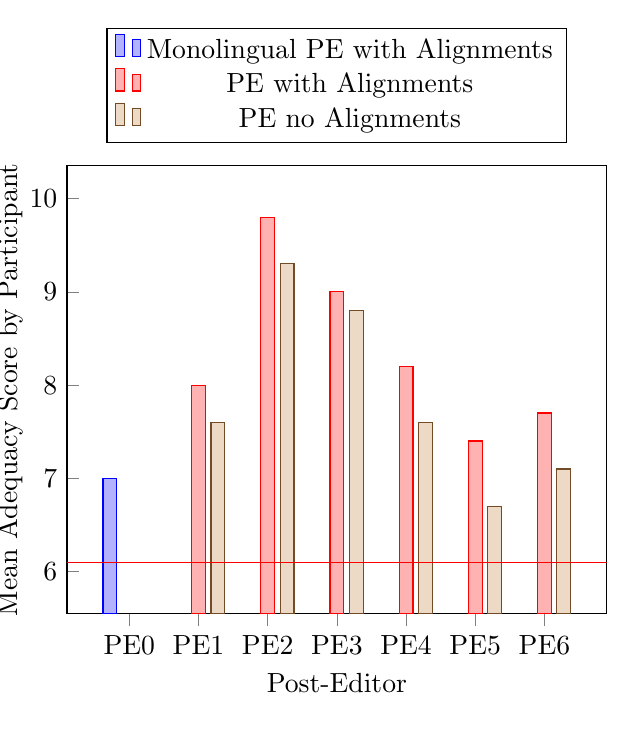
\begin{tikzpicture}[trim left={(-0.5,0)},trim axis right]
\begin{axis}[%scale only axis=true, width=80mm, height=73mm,
    ybar,
    enlargelimits=0.15,
    legend style={at={(0.5,1.05)},anchor=south},
   ylabel={Mean Adequacy Score by Participant},
   xlabel={Post-Editor},
   % symbolic x coords={PE0,PE1,PE2,PE3,PE4,PE5,PE6},
    xtick={0,1,2,3,4,5,6},
    xticklabels={PE0,PE1,PE2,PE3,PE4,PE5,PE6},
	xtick pos=left,
	ytick pos=left,
	ylabel shift={-0.15cm},
    %xtick=data,
    %nodes near coords,
    %nodes near coords align={vertical},
    bar width=5pt
    ]

\addplot coordinates { (0,7.0) (0,6.1)};
\addplot coordinates { (1,8.0) (2,9.8) (3,9.0) (4,8.2) (5,7.4) (6,7.7)};
\addplot coordinates { (1,7.6) (2,9.3) (3,8.8) (4,7.6) (5,6.7) (6,7.1)};

\addplot[red,sharp plot,update limits=false] 
	coordinates {(-1,6.1) (8,6.1)};
	%node[above] at (axis cs:3,6.1) {Unedited MT};
	
%%\addplot coordinates {(tool8,1) (tool9,1) (tool10,1)};
\legend{Monolingual PE with Alignments, PE with Alignments,PE no Alignments}
\end{axis}
\end{tikzpicture}
\caption{Russian-English}
\label{fig:mean_adequacy_score_per_posteditor_ru}
\end{center}
\end{subfigure}
\ \\ \ \\
\begin{subfigure}[b]{\linewidth}
\begin{center}
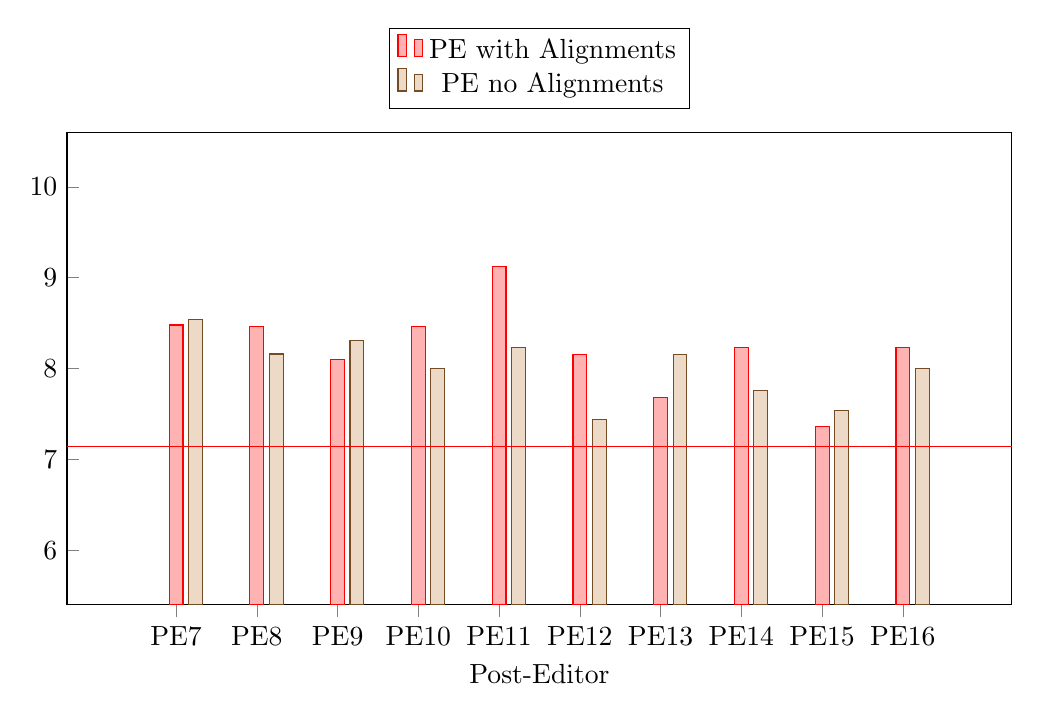
\begin{tikzpicture}[trim left={(-0.5,0)},trim axis right]
\begin{axis}[scale only axis=true, width=120mm, height=60mm,
    ybar,
    enlargelimits=0.15,
    legend style={at={(0.5,1.05)},anchor=south},
%   ylabel={Mean Adequacy Score by Participant},
   xlabel={Post-Editor},
   % symbolic x coords={PE0,PE1,PE2,PE3,PE4,PE5,PE6},
    xtick={1,2,3,4,5,6,7,8,9,10},
    xticklabels={PE7,PE8,PE9,PE10,PE11,PE12,PE13,PE14,PE15,PE16},
	xtick pos=left,
	ytick pos=left,
	ylabel shift={-0.15cm},
	ymin=6,
	ymax=10,
    %xtick=data,
    %nodes near coords,
    %nodes near coords align={vertical},
    bar width=5pt
    ]

%	Adequacy with align	Adequacy w/o align
%PE7	8.48	8.54
%PE8	8.46	8.16
%PE9	8.1	8.31
%PE10	8.46	8
%PE11	9.12	8.23
%PE12	8.15	7.44
%PE13	7.68	8.15
%PE14	8.23	7.76
%PE15	7.36	7.54
%PE16	8.23	8
%		
%Note overall mean for MT is 7.14		

\addplot coordinates {};
\addplot coordinates {(1,8.48) (2,8.46) (3,8.1) (4,8.46) (5,9.12) (6,8.15) (7,7.68) (8,8.23) (9,7.36) (10,8.23) };
\addplot coordinates {(1,8.54) (2,8.16) (3,8.31) (4,8) (5,8.23) (6,7.44) (7,8.15) (8,7.76) (9,7.54) (10,8) };
%\addplot coordinates {(1,8.8) (2,8.461538461538462) (3,8.56) (4,8.76923076923077) };
%\addplot coordinates {(1,8.23076923076923) (2,8.72) (3,8.461538461538462) (4,8.88) };
\addplot[red,sharp plot,update limits=false] coordinates { (-1,7.14) (12,7.14) };

%%\addplot coordinates {(tool8,1) (tool9,1) (tool10,1)};
\legend{PE with Alignments,PE no Alignments}
\end{axis}
\end{tikzpicture}
\end{center}
\caption{Spanish-English}
\label{fig:mean_adequacy_score_per_posteditor_es}
\end{subfigure}
\caption{Mean adequacy score per post-editor. The red horizontal line indicates the mean adequacy score (Russian-English: 6.1; Spanish-English: 7.1) of the unedited MT.}
\label{fig:mean_adequacy_score_per_posteditor}
\end{figure}
